\section{Zadanie 2: Analiza metod numerycznych}

\subsection{Charakterystyka metod i problem}
W ramach tego zadania przeanalizowano działanie wybranych metod numerycznych, takich jak metoda bisekcji, metoda falsi, metoda Newtona-Raphsona oraz metoda siecznych, pod kątem znajdowania miejsc zerowych funkcji. Każda z metod została opisana w kontekście założeń, wyprowadzenia wzoru oraz implementacji algorytmu.

\subsubsection{Metoda bisekcji}
Metoda bisekcji jest jedną z najprostszych metod numerycznych do znajdowania miejsc zerowych funkcji.

\begin{itemize}
    \item Założenia:
    \begin{itemize}
        \item Funkcja \( f(x) \) jest ciągła na przedziale \([a, b]\).
        \item Istnieje co najmniej jedno miejsce zerowe w przedziale \([a, b]\), tj. \( f(a) \cdot f(b) < 0 \).
    \end{itemize}
    \item Wzór:
    \[ c = \frac{a + b}{2} \]
    \item Wyprowadzenie:
    Metoda polega na iteracyjnym dzieleniu przedziału \([a, b]\) na połowy. W każdym kroku wybierany jest podprzedział, który zawiera miejsce zerowe, na podstawie znaku iloczynu \( f(a) \cdot f(c) \). Proces jest kontynuowany aż do osiągnięcia zadanej dokładności \( \text{acc} \).
\end{itemize}

\subsubsection{Metoda falsi}
Metoda falsi wykorzystuje prostą do znajdowania miejsc zerowych na podstawie wartości funkcji na krańcach przedziału.

\begin{itemize}
    \item Założenia:
    \begin{itemize}
        \item Funkcja \( f(x) \) jest ciągła na przedziale \([z_1, z_2]\).
        \item \( f(z_1) \cdot f(z_2) < 0 \).
    \end{itemize}
    \item Wzór:
    \[ c = \frac{a \cdot f(b) - b \cdot f(a)}{f(b) - f(a)} \]
    \item Wyprowadzenie:
    Metoda zakłada, że miejsce zerowe funkcji można przybliżyć prostą przechodzącą przez punkty \((a, f(a))\) i \((b, f(b))\). Nowy punkt \( c \) jest obliczany jako przecięcie tej prostej z osią \( x \) ($f(c) = 0$).
    \[
     \frac{-f(a)}{c-a} = \frac{f(c) - f(a)}{c-a} = \frac{f(b) - f(a)}{b-a}
    \]
    przekształcając otrzymujemy
    \[ c = \frac{a \cdot f(b) - b \cdot f(a)}{f(b) - f(a)} \]
    Proces jest powtarzany, aż różnica między kolejnymi przybliżeniami osiągnie zadaną dokładność.
\end{itemize}

\subsubsection{Metoda Newtona-Raphsona}
Metoda Newtona-Raphsona jest szybką metodą iteracyjną wykorzystującą pochodne funkcji.

\begin{itemize}
    \item Założenia:
    \begin{itemize}
        \item Funkcja \( f(x) \) jest różniczkowalna w otoczeniu miejsca zerowego.
        \item Znany jest punkt startowy \( x_0 \), który jest blisko miejsca zerowego.
    \end{itemize}
    \item Wzór:
    \[ x_{i+1} = x_i - \frac{f(x_i)}{f'(x_i)} \]
    \item Wyprowadzenie:
    Metoda wykorzystuje rozwinięcie funkcji w szereg Taylora w punkcie \( x_i \). 
    \[
    f(x) \sim f(x_0) + f'(x_0)(x - x_0) 
    \]
    Co po przekształceniu i założeniu że $(f(x) = 0)$ daje:
    \[
    x = x_0 - \frac{f(x_0)}{f'(x_0)}
    \]
    Przecięcie stycznej do funkcji w punkcie \( x_i \) z osią \( x \) daje kolejne przybliżenie \( x_{i+1} \). Proces iteracji kontynuuje się, aż do spełnienia warunku \( |f(x_{i+1})| < \text{acc} \).
\end{itemize}

\subsubsection{Metoda siecznych}
Metoda siecznych jest modyfikacją metody Newtona-Raphsona, w której nie wymaga się obliczania pochodnych funkcji.

\begin{itemize}
    \item Założenia:
    \begin{itemize}
        \item Funkcja \( f(x) \) nie musi być różniczkowalna.
        \item Znane są dwa punkty startowe \( x_0 \) i \( x_1 \).
    \end{itemize}
    \item Wzór:
    \[ x_{i+1} = x_i - \frac{f(x_i)(x_i - x_{i-1})}{f(x_i) - f(x_{i-1})} \]
    \item Wyprowadzenie:
    Zamiast stycznej wykorzystuje się cięciwę przechodzącą przez dwa kolejne punkty \((x_{i-1}, f(x_{i-1}))\) i \((x_i, f(x_i))\). Zatem wystarczy po prostu rozpisać pochodną z definicji i wstawić odpowiednie wartości.
\end{itemize}

\subsection{Przeprowadzone testy}
Przeprowadzono dwa rodzaje testów dla każdej z metod:

\begin{itemize}
    \item Analiza zmiany błędu w zależności od liczby iteracji, od (2-20 i 2-120). 
    \item Wyznaczenie liczby iteracji i czasu potrzebnego do osiągnięcia zadanej dokładności \(\in [10^{-1}, 10^{-32}\). (Maksymalna liczba iteracji $=1000$) 
\end{itemize}

Funkcje testowe:\
\begin{itemize}
    \item \( \text{Pol } x=0.23 \): \( f(x) = (x - 0.23)(x + 1)(x + 2)(x + 3)(x + 4) \)
    \item \( \text{Pol } x=0.53 \): \( f(x) = (x - 0.53)(x + 1)(x + 2)(x + 3)(x + 4) \)
\end{itemize}
Dla każdej funkcji analizowano przypadki, gdy punkt startowy znajduje się bliżej środka przedziału oraz bliżej jego skrajnej wartości.

{\centering
\paragraph{Wzrost błędu}
\indent

\paragraph{Przedział \([0, 1]\)}
\indent

\begin{minipage}{0.48\textwidth}
    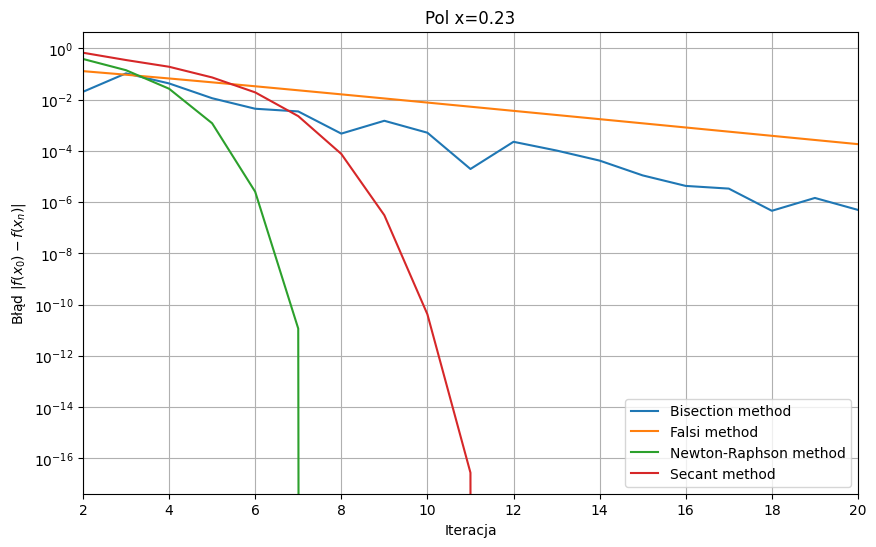
\includegraphics[width = \textwidth]{wykresy/zad2_error_rising/0_1/20_x_0_23.png}
\end{minipage}
\begin{minipage}{0.48\textwidth}
    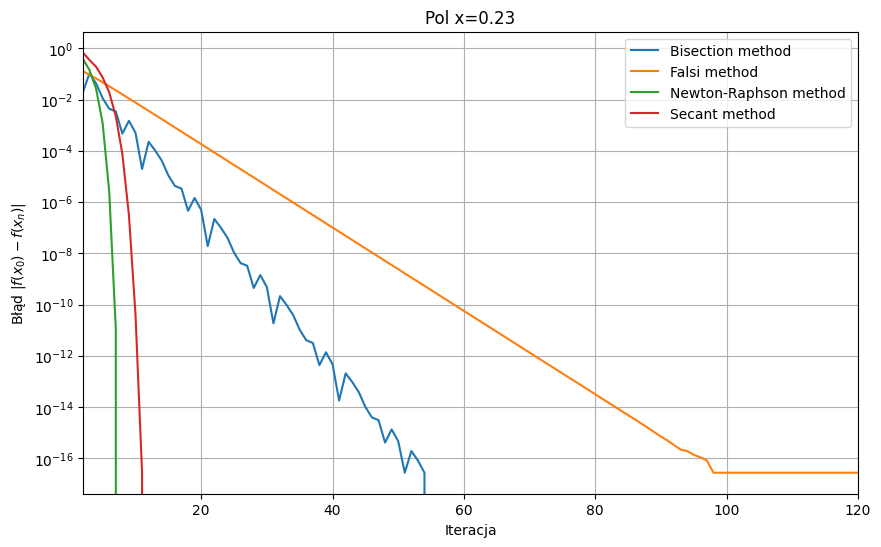
\includegraphics[width = \textwidth]{wykresy/zad2_error_rising/0_1/120_x_0_23.png}
\end{minipage}
Wielomian z $x_0 = 0.23$

\begin{minipage}{0.48\textwidth}
    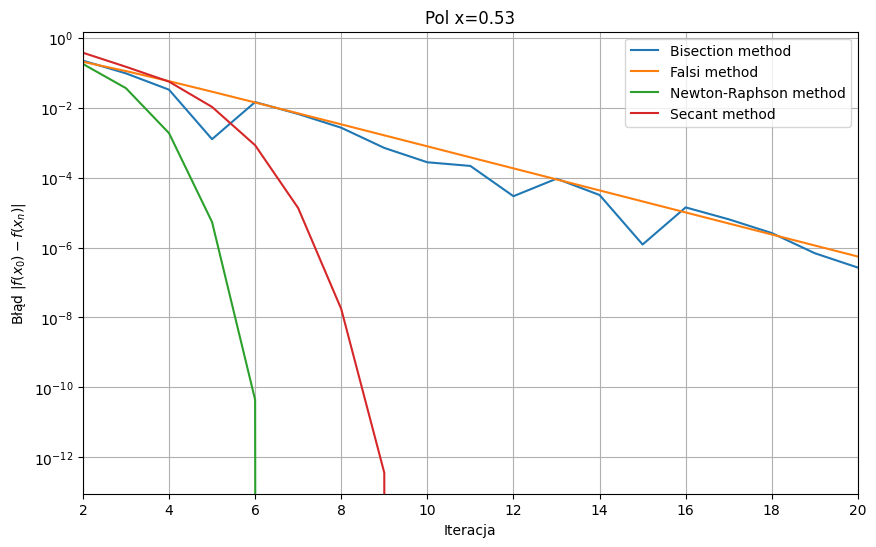
\includegraphics[width = \textwidth]{wykresy/zad2_error_rising/0_1/20_x_0_53.png}
\end{minipage}
\begin{minipage}{0.48\textwidth}
    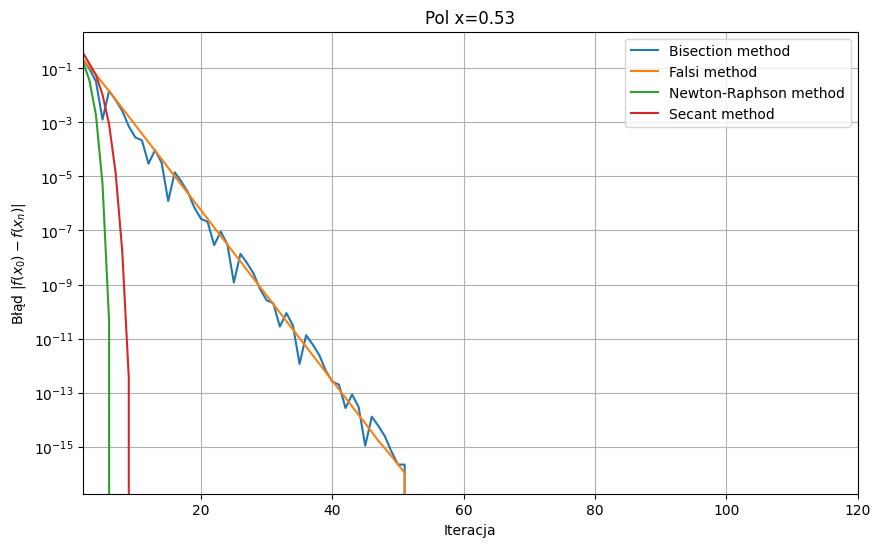
\includegraphics[width = \textwidth]{wykresy/zad2_error_rising/0_1/120_x_0_53.png}
\end{minipage}
Wielomian z $x_0 = 0.53$

\paragraph{Przedział \([0, 100]\)}
\indent

\begin{minipage}{0.48\textwidth}
    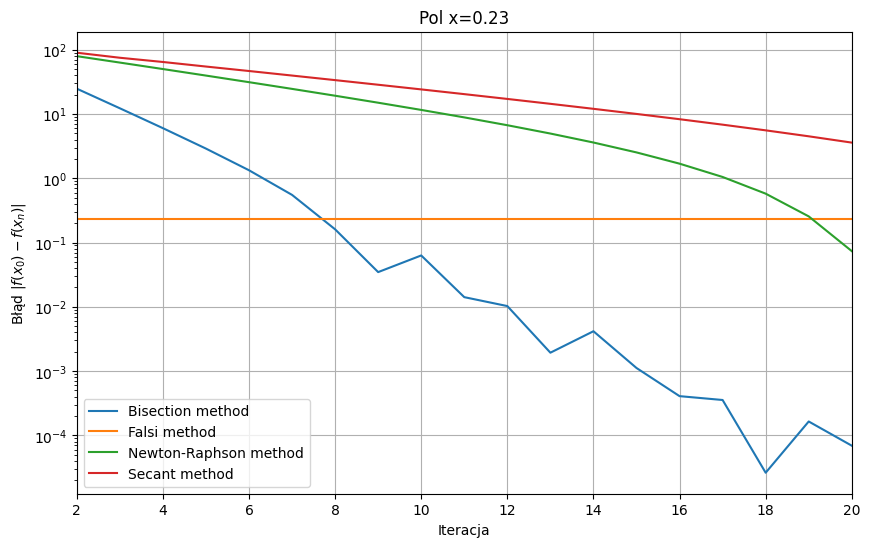
\includegraphics[width = \textwidth]{wykresy/zad2_error_rising/0_100/20_x_0_23.png}
\end{minipage}
\begin{minipage}{0.48\textwidth}
    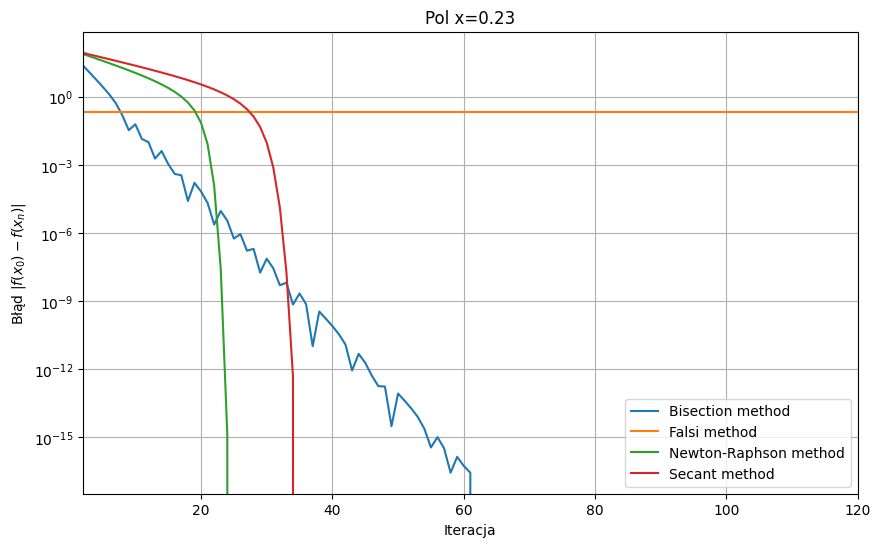
\includegraphics[width = \textwidth]{wykresy/zad2_error_rising/0_100/120_x_0_23.png}
\end{minipage}
Wielomian z $x_0 = 0.23$

\begin{minipage}{0.48\textwidth}
    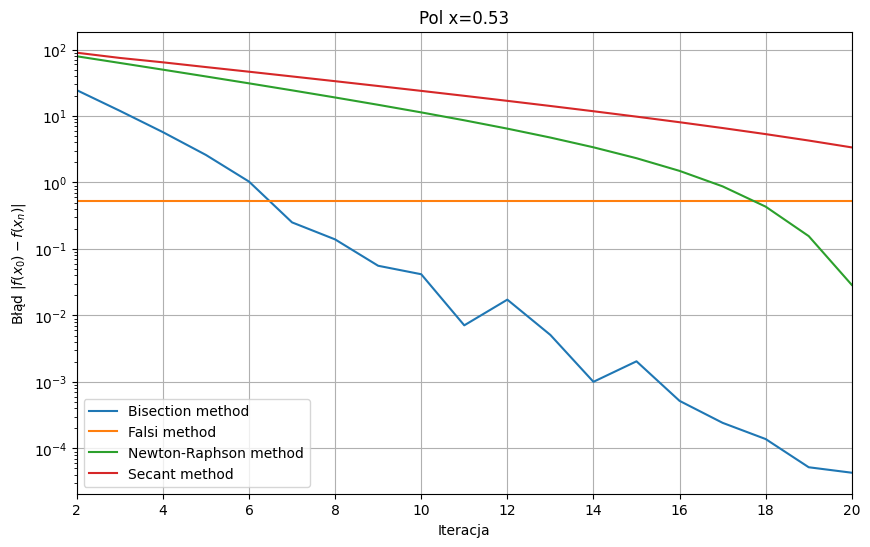
\includegraphics[width = \textwidth]{wykresy/zad2_error_rising/0_100/20_x_0_53.png}
\end{minipage}
\begin{minipage}{0.48\textwidth}
    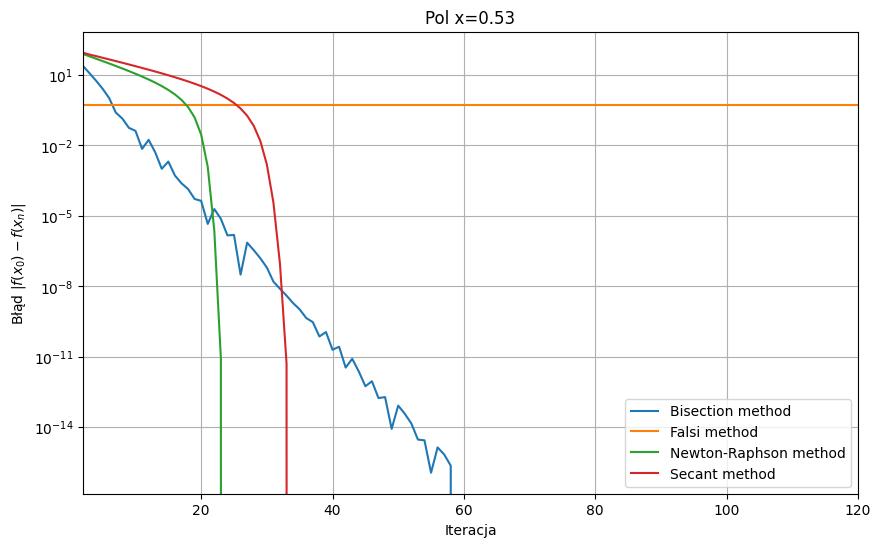
\includegraphics[width = \textwidth]{wykresy/zad2_error_rising/0_100/120_x_0_53.png}
\end{minipage}
Wielomian z $x_0 = 0.53$

}

{\centering
\paragraph{Osiągnięcie wymaganej dokładności}
\indent

\paragraph{Przedział \([0, 1]\)}
\indent

\begin{minipage}{0.48\textwidth}
    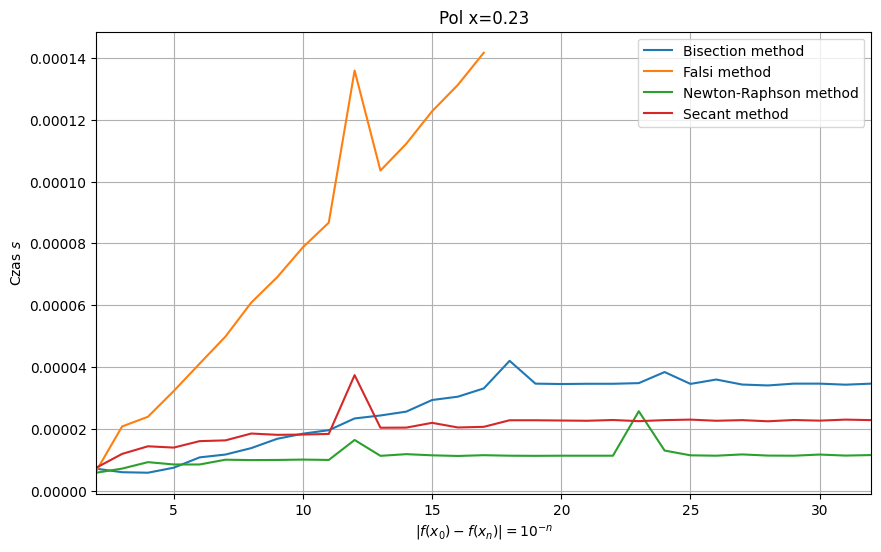
\includegraphics[width = \textwidth]{wykresy/zad2_accuracy_till/0_1/time_023.png}
\end{minipage}
\begin{minipage}{0.48\textwidth}
    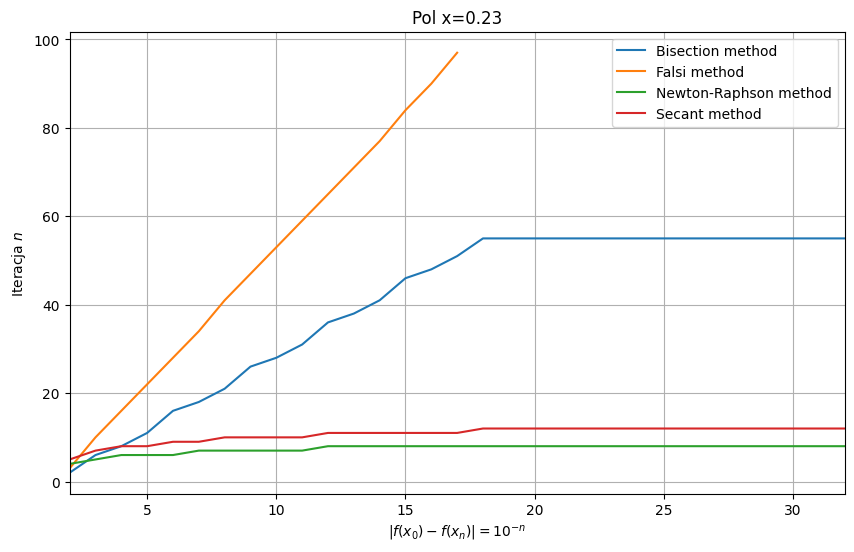
\includegraphics[width = \textwidth]{wykresy/zad2_accuracy_till/0_1/iteration_023.png}
\end{minipage}
Wielomian z $x_0 = 0.23$

\begin{minipage}{0.48\textwidth}
    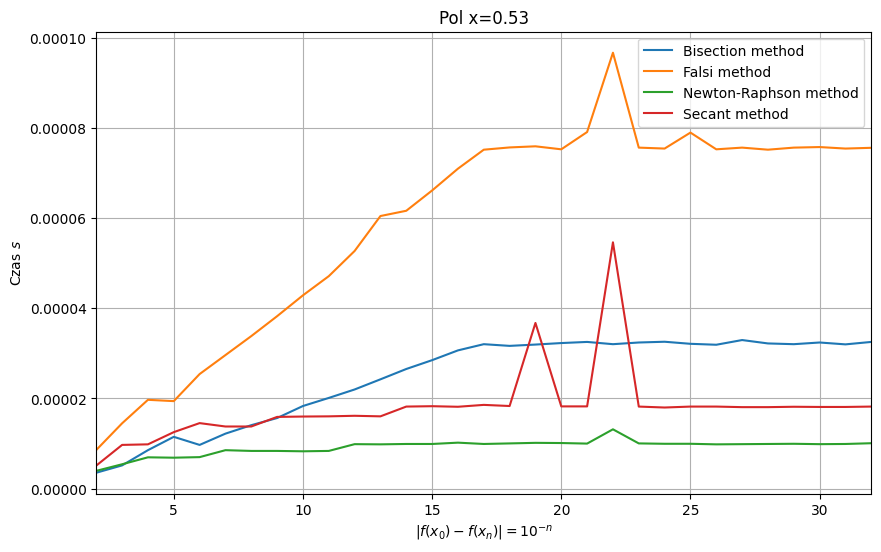
\includegraphics[width = \textwidth]{wykresy/zad2_accuracy_till/0_1/time_053.png}
\end{minipage}
\begin{minipage}{0.48\textwidth}
    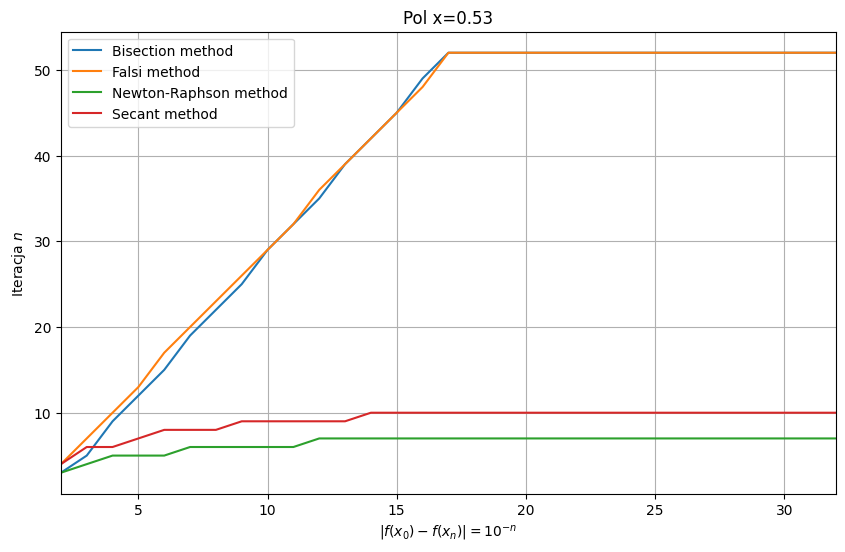
\includegraphics[width = \textwidth]{wykresy/zad2_accuracy_till/0_1/iteration_053 .png}
\end{minipage}
Wielomian z $x_0 = 0.53$

\paragraph{Przedział \([0, 100]\)}
\indent

\begin{minipage}{0.48\textwidth}
    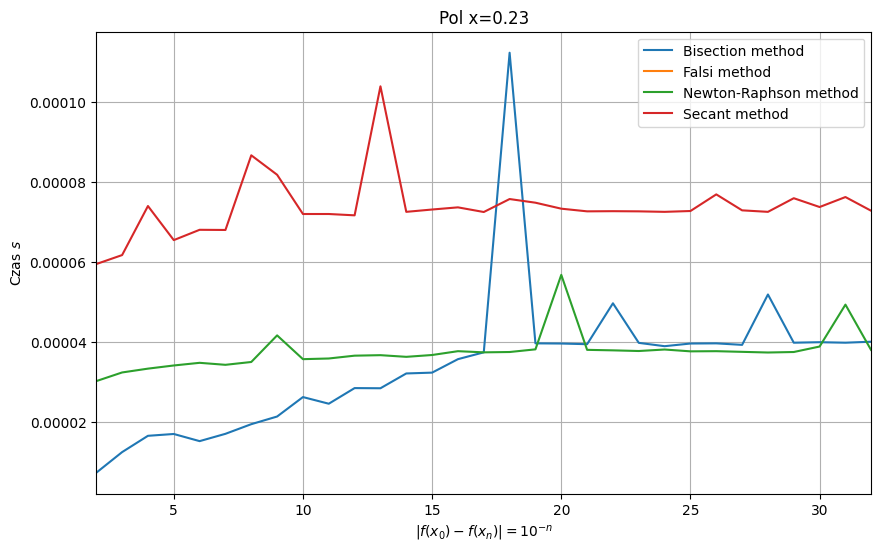
\includegraphics[width = \textwidth]{wykresy/zad2_accuracy_till/0_100/time_023.png}
\end{minipage}
\begin{minipage}{0.48\textwidth}
    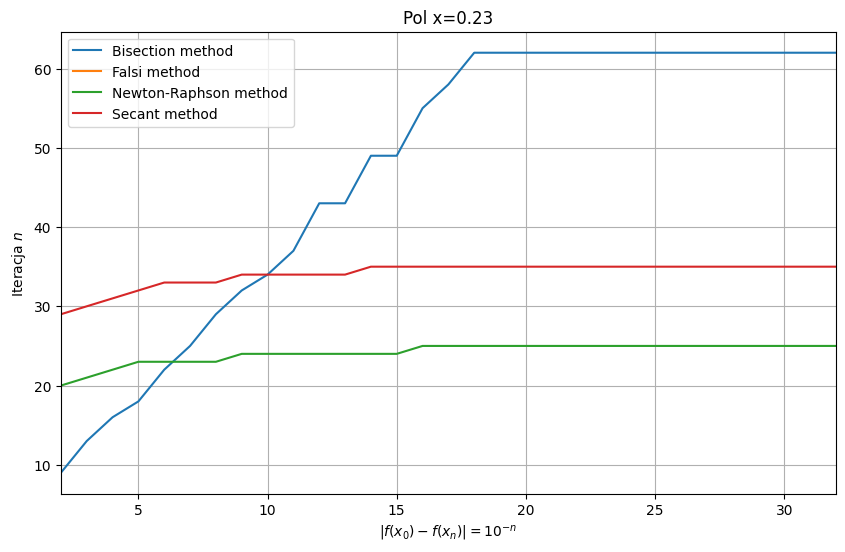
\includegraphics[width = \textwidth]{wykresy/zad2_accuracy_till/0_100/iteration_023.png}
\end{minipage}
Wielomian z $x_0 = 0.23$

\begin{minipage}{0.48\textwidth}
    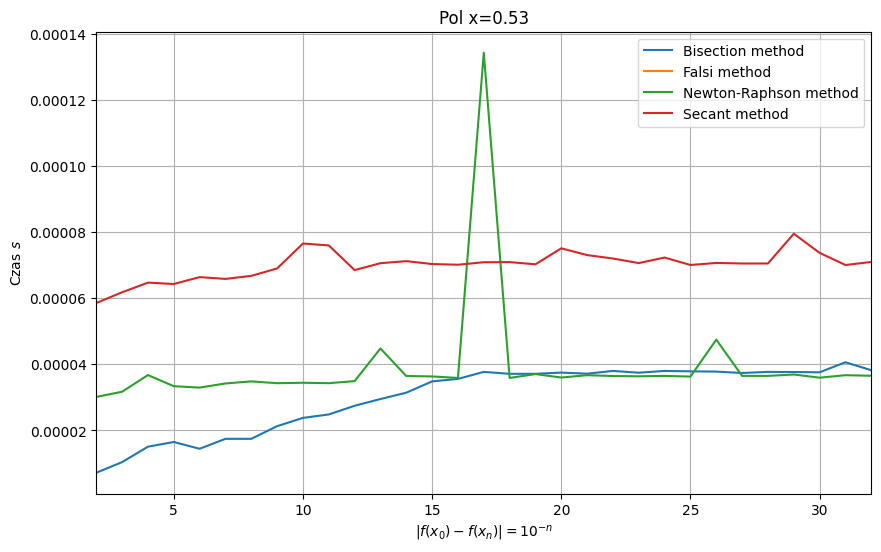
\includegraphics[width = \textwidth]{wykresy/zad2_accuracy_till/0_100/time_053.png}
\end{minipage}
\begin{minipage}{0.48\textwidth}
    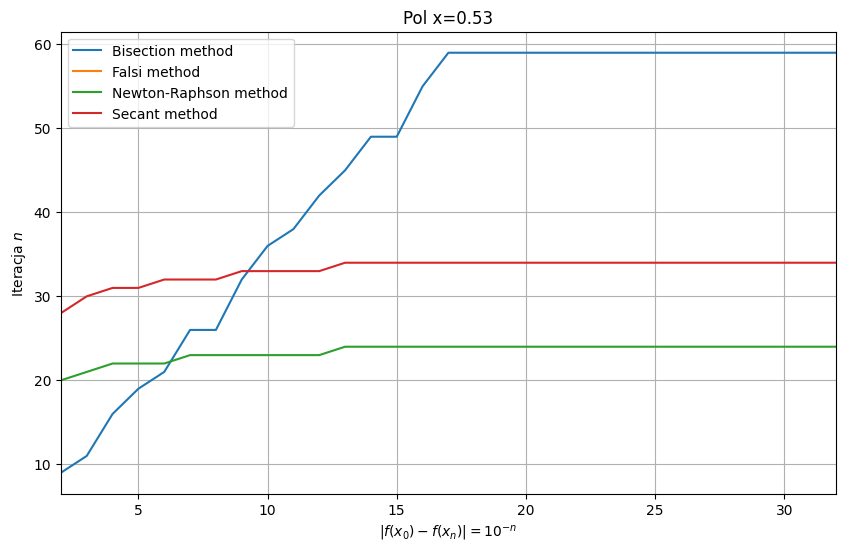
\includegraphics[width = \textwidth]{wykresy/zad2_accuracy_till/0_100/iteration_053.png}
\end{minipage}
Wielomian z $x_0 = 0.53$

}


\subsection{Wnioski i analiza}
\paragraph{Zmiana błędu w zależności od liczby iteracji}
\begin{itemize}
\item Metoda Newtona-Raphsona, choć wymaga początkowego punktu blisko miejsca zerowego, jest najszybsza. Błąd zmniejsza się wykładniczo, co czyni ją bardzo efektywną.
\item Metoda secant jest wolniejsza niż Newtona-Raphsona, ale pozwala na aproksymację funkcji nieróżniczkowalnych. Jej dokładność również rośnie wykładniczo, choć z mniejszym współczynnikiem zbieżności.
\item Metoda falsi redukuje błąd w sposób liniowy, jednakże dla miejsc zerowych, które są ekstremalnie blisko jednego z końców, metoda ta okazuje się nieskuteczna. Czas jej działania jest gorszy lub porównywalny do metody bisekcji. To może wynikać z faktu, że funkcje testowe były wyjątkowo nieodpowiednio dobrane do tej metody, która proponuje statystyczne rozwiązanie i powinna być bardziej efektywna.
\end{itemize}

\paragraph{Ilość iteracji i czas potrzebny do osiągnięcia precyzji}
\begin{itemize}
\item Dla metod bisekcji i falsi czas oraz liczba iteracji rosną liniowo wraz ze wzrostem wymaganej precyzji.
\item Dla metod Newtona-Raphsona i secant liczba iteracji i czas są stałe po osiągnięciu miejsca zerowego.
\item Na dużym przedziale metoda falsi była nieefektywna, a nawet nie zbieżna, co czyniło ją nieużyteczną w takich przypadkach.
\end{itemize}

